\subsection{Problem setup}
	{\nologo
	\begin{frame}{Problem setup: hypothesis}
	\begin{alertblock}{Hypothesis}
		\begin{itemize}
			\item \textbf{not using} an \textbf{inlet guide vane} for simplicity of design\footnote{$V_{t0} = 0 \frac{m}{s}$ and $\chi$ dictate the behaviour of $\lambda$.}
			\item keeping, in the similarity/adimensional analysis of the compressor, $V_{a_{mean}}$ \textbf{constant}\footnote{$\dot{m}$ corrections will be made later on in the \textbf{radial equilibrium} solution.}  
			\item keeping the blade height, $b_0$, \textbf{constant} both in rotor and stator\footnote{In order to keep each \textbf{blade streamtube section} as simple as possible.}
			\item using a \textbf{free vortex} model for the velocity triangles
			\item neglecting inlet \textbf{entropy} generation and assuming \textbf{rotor inlet} quantities \textbf{constant}
			\item \textbf{shrouding} at blade tip not present
			\item \textbf{rotor-stator} losses neglected
		\end{itemize}
	\end{alertblock}
	\end{frame}
	}
		\begin{frame}{Problem setup: solution steps}
		\begin{block}{Main procedural steps:}
			\begin{itemize}
				\item $\lambda$ and $\psi$ computation from $\chi$ and $V_{t0}$
				\item $\phi$ and $\eta$ computation 
				\item $V_{a_{mean}}$ and $L_{eu}$ computation from $\phi$, $\beta_{TT}$ and $\eta$
				\item computing \textbf{mean} velocity triangles, using the above hypothesis
				\item computing \textbf{mean thermodynamic} quantities 
				\item computing \textbf{blade height}
			\end{itemize}
		\end{block}
	\end{frame}
\subsection{Main design quantities}
	\begin{frame}{Graph Analysis: $\chi$ \& $M$}
		\begin{figure}
			\centering
			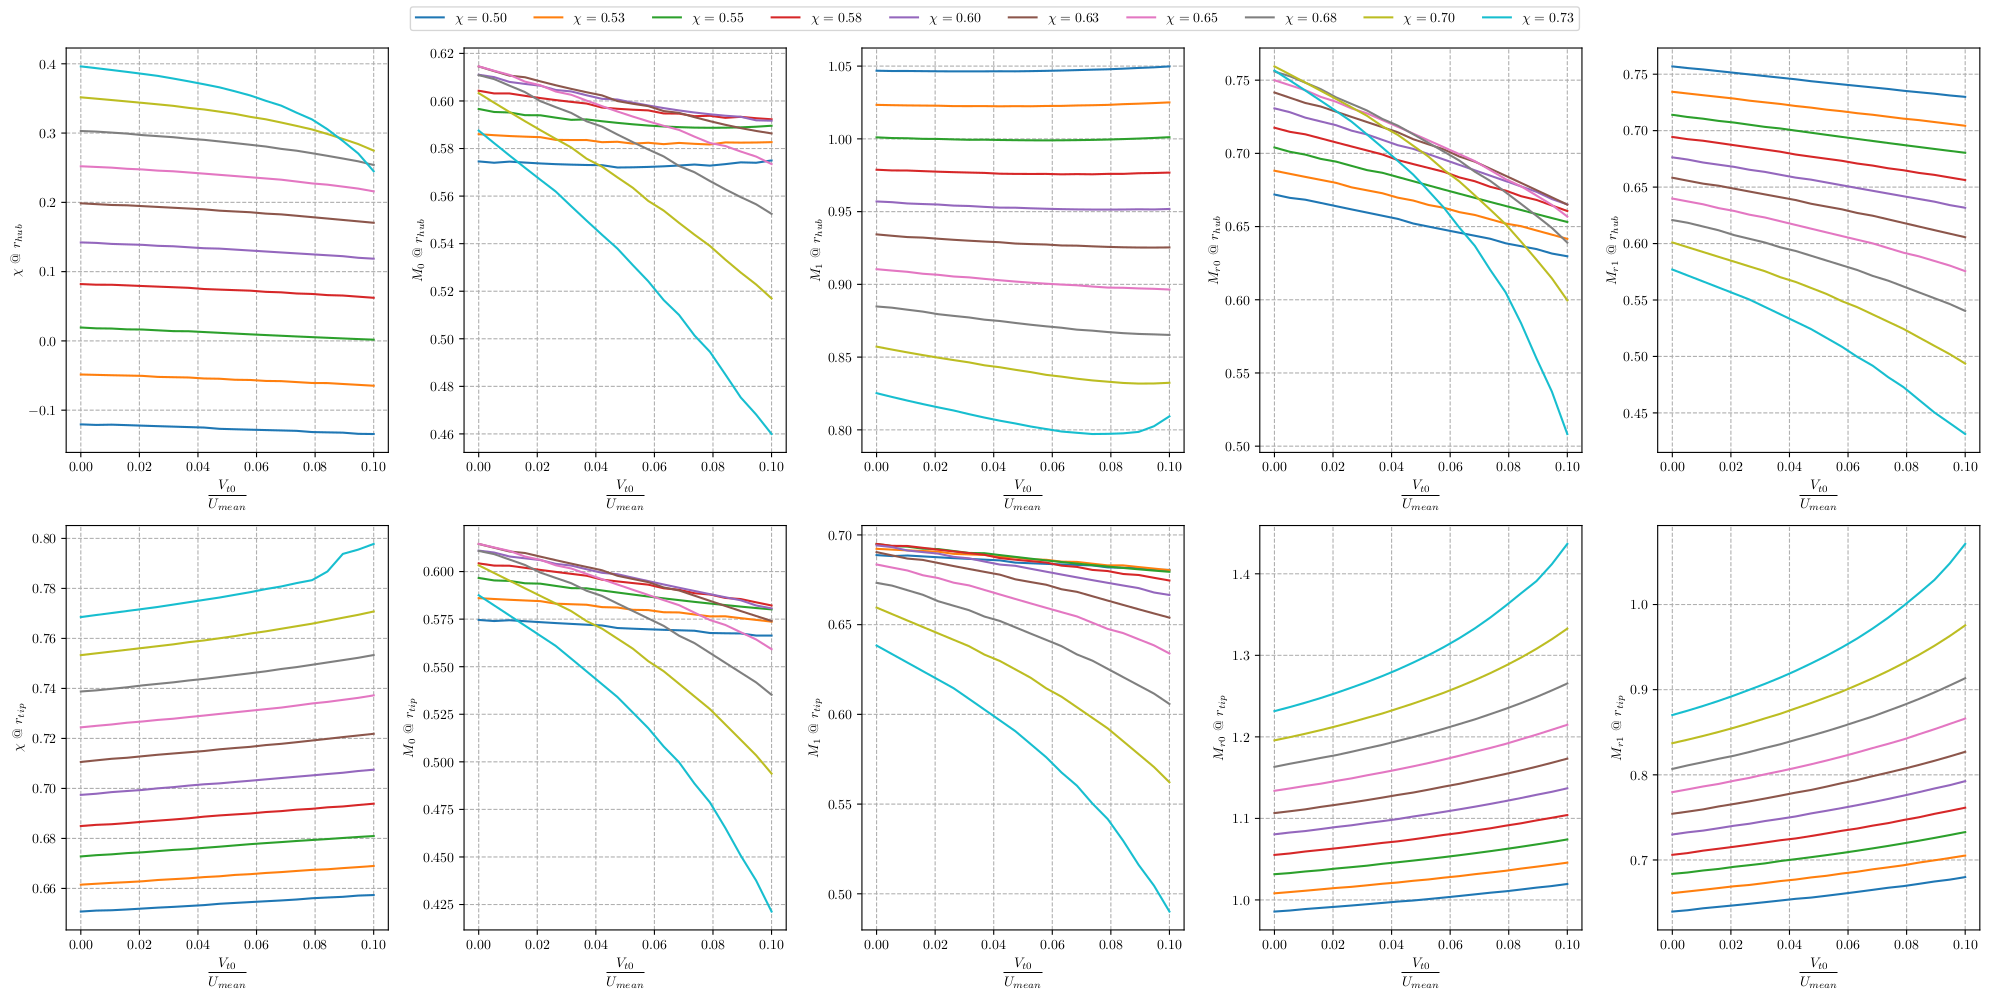
\includegraphics[width=\textwidth]{figures/reactionStudy0.png}
		\end{figure}
	\end{frame}
	\begin{frame}{Graph Analysis: $\alpha$ \& $\beta$}
		\begin{figure}
			\centering
			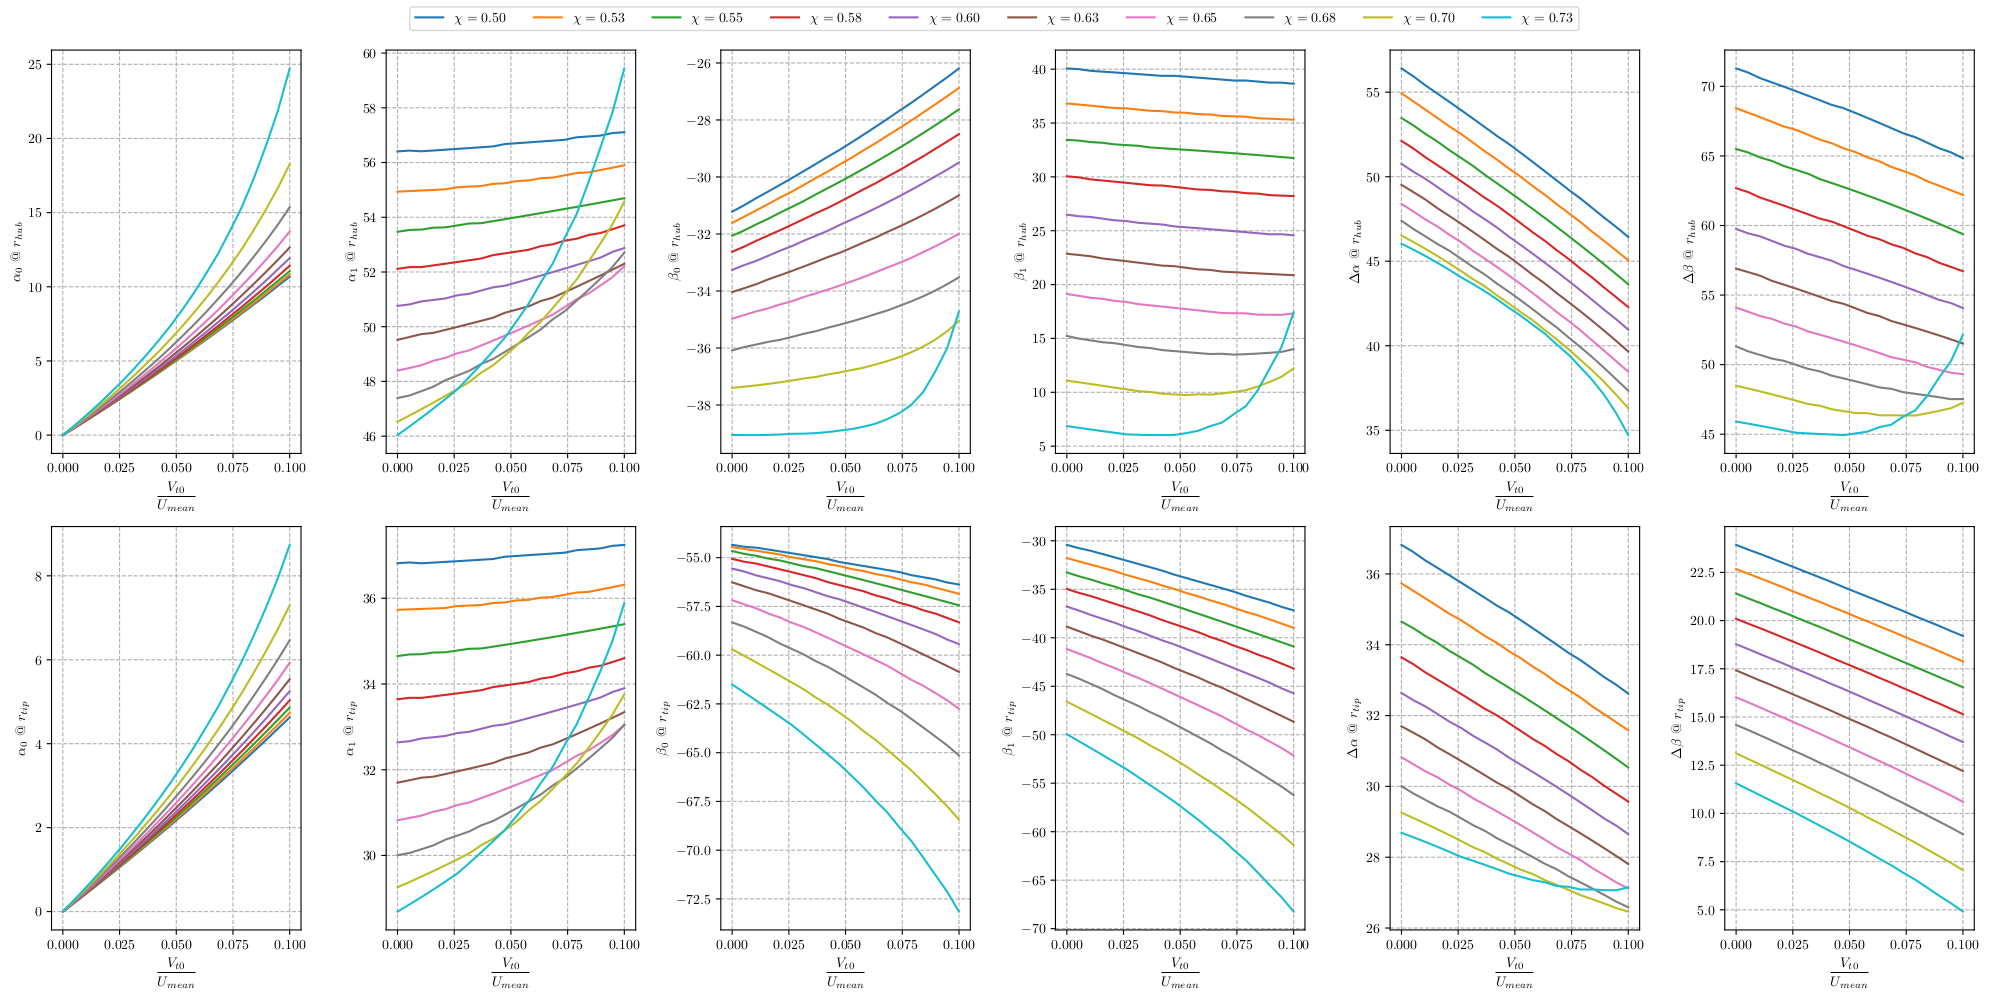
\includegraphics[width=\textwidth]{figures/reactionStudy1.png}
		\end{figure}
	\end{frame}
	\begin{frame}{$\lambda$ \& $\psi$}
		From the previous \textbf{graphs}:
			\begin{itemize}
				\item $\chi = 0.55$
				\item $r_{mean} = 0.325 m$
				\item $\frac{V_{t0}}{U_{mean}} = 0$
			\end{itemize}
		Taking into account the previous modeling \textbf{hypothesis}:
		\begin{align}
			\lambda & = \Bigg( 1 - \chi - \frac{V_{t0}}{U_{mean}} \Bigg) \cdot 4 \nonumber \\
			\psi    & = \frac{\lambda}{2} \nonumber
		\end{align}
	\end{frame}
	
	\begin{frame}{$\phi_{(\psi)}$}
		From \cite[Sec. 10.4]{axial2004} it is imposed that $\frac{W_2}{W_1} \geq 0.7$ with a \textit{safety} margin of $3 \%$.  
		\begin{figure}
			\centering
			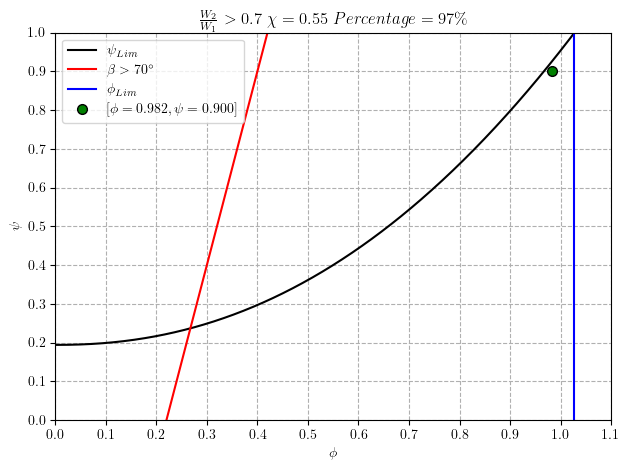
\includegraphics[width=0.7\textwidth]{figures/stagePerf.png}
		\end{figure}
	\end{frame}
	\begin{frame}{$\eta$ \& $L_{eu}$}
		$\eta$ is computed from an \textbf{Lieblein} efficiency chart\footnote{This chart has been interpolated from the course slides charts.} given $\phi$ and $\chi$. This parameter will be used for the computation of $L_{eu}$ given the $\beta_{TT}$ target.
		\begin{columns}
			\column{0.5\textwidth}
				\begin{figure}
					\centering 
					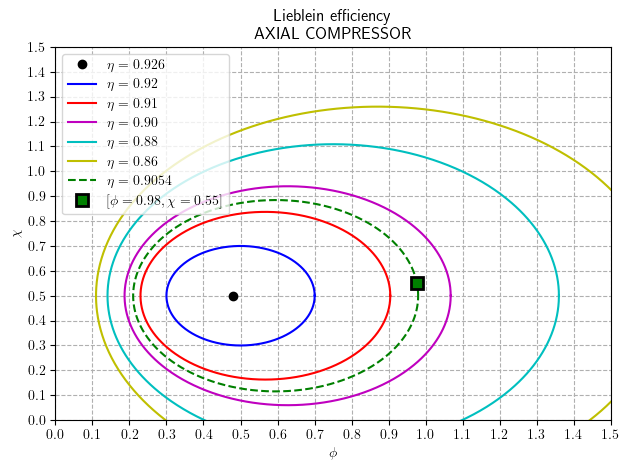
\includegraphics[width=1\textwidth]{figures/efficiency.png}
				\end{figure}
			\column{0.5\textwidth}
			\begin{align}
				L_{is} & = \frac{\gamma \ R}{\gamma - 1} \ T_{in} \ (\beta_{TT}^{{\frac{\gamma - 1}{\gamma}}} - 1) \nonumber \\
				L_{eu} & = \frac{L_{is}}{\eta} \nonumber
			\end{align}
		\end{columns}
	\end{frame}
\subsection{$V_{t_{mean}}$, $V_{a_{mean}}$, $U_{mean}$ \& velocity triangles}
\begin{frame}[fragile]{$V_{a_{mean}}$, $V_{t_{mean}}$ \& $U_{mean}$}
	\begin{align}
		U_{mean} & = \frac{L_{eu}}{\psi} \nonumber \\ 
		V_{a_{mean}} & = \phi \ U_{mean} \nonumber \\
		L_{eu} & = U_1 \ V_{t1} - U_0 \ V_{t0} \nonumber \\ 
		       & = U_{1_{mean}} \ V_{t1_{mean}} - U_{0_{mean}} \ V_{t0_{mean}} = U_{mean} \ \Delta V_{t_{mean}} \nonumber \\
		V_{t1} & = \Delta V_{t_{mean}} + V_{t0} \nonumber  
	\end{align}
	\begin{itemize}
		\item $\Delta V_{t_{mean}}$ computation allows to get a \textit{first sketch} of the \textbf{velocity triangles}\footnote{\textbf{Free vortex} model based.}
		\item The first analysis results are stored in \verb|compressor_0.55_0.325_28_28.txt|
	\end{itemize}
\end{frame}

{\nologo
\begin{frame}
	\begin{columns}
		\column{0.5\textwidth}
			\begin{figure}
				\centering
				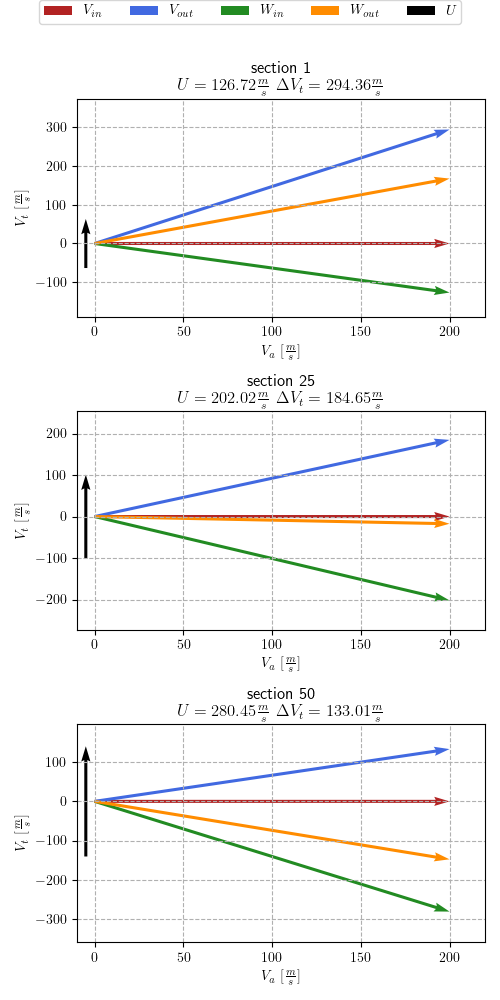
\includegraphics[width=0.7\textwidth]{figures/rotorVelocityTriangle.png}
			\end{figure}
		\column{0.5\textwidth}
			\begin{figure}
				\centering
				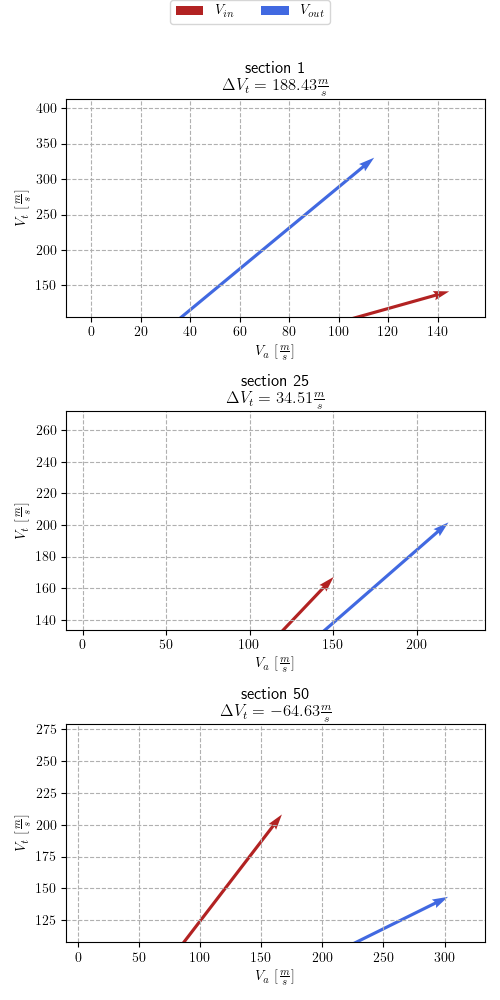
\includegraphics[width=0.7\textwidth]{figures/statorVelocityTriangle.png}
			\end{figure}
	\end{columns}
\end{frame}
}

